\documentclass{standalone}
\usepackage{tikz}
\begin{document}
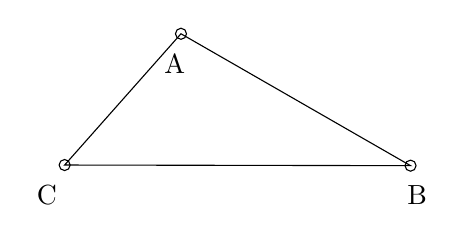
\begin{tikzpicture}[x=1pt,y=1pt]
\draw (229.94,-197.39) -- (104.95,-197.16) -- (146.99,-149.73) -- cycle;
\node at (144.71,-160.72) {A};
\node at (232.33,-207.90) {B};
\node at (98.54,-207.90) {C};
\draw (146.99,-149.73) circle (2.00);
\draw (229.94,-197.39) circle (2.00);
\draw (104.95,-197.16) circle (2.00);
\end{tikzpicture}
\end{document}
